%% Page settings.
\documentclass[10pt,a4paper,twoside]{article}
\usepackage[top=1.5in, left=1.2in, bottom=1.5in, right=1.2in]{geometry}
%==================================================%
%% Encoding packages.
\usepackage[UKenglish]{babel}
\usepackage[nodayofweek]{datetime}
\usepackage[T1]{fontenc}
\usepackage[utf8]{inputenc}
\usepackage{amsmath}
\usepackage{amsthm}
\usepackage{amsfonts}
\usepackage{amssymb}
\usepackage{calc}
\usepackage{natbib}
\usepackage{color}
\usepackage{subcaption}
%==================================================%
%% Document details.
\usepackage{titling}
\title{Information and admissible sets}
\author{Jeff Rowley}
\newcommand{\thedate}{\today}
% Enter document details here.
\newcommand{\details}{C:/Dropbox/TeXTemplates/}
% Enter the file path here for the UCL logo and bibliography.
% Change this file path for different computer systems.
%==================================================%
%% Date macro.
\newcommand{\theseason}[1]{
\ifcase \month 
\or Winter\or Winter\or Spring\or Spring\or Spring\or Summer\or Summer\or Summer\or Autumn\or Autumn\or Autumn\or Winter\fi}
% Displays the season.
% Obsolete in this template.
%==================================================%
%% Useful packages.
\usepackage{enumerate}		% Lists.
\usepackage{bbm}			% Indicator functions.
\usepackage{lipsum}			% Random text generator.
\usepackage{MnSymbol}		% Arrows.
\usepackage{graphicx}		% Graphics.
%==================================================%
%% Theorem environments.
\newcounter{countthm}[section]
\newcounter{countlem}[section]
\newcounter{countex}[section]
% Creates new counters which reset at each new section. 
\renewcommand{\thecountthm}{\thesection.\arabic{countthm}}
\renewcommand{\thecountlem}{\thesection.\arabic{countlem}}
\renewcommand{\thecountex}{\thesection.\arabic{countex}}
% Redefines counters to include the section number.
\newtheorem{thm}[countthm]{Theorem}
% Creates a theorem environment - type \thm to begin.
\newtheorem{lem}[countlem]{Lemma}
% Creates a lemma environment - type \lem to begin.
\newtheorem{ex}[countex]{Example}
% Creates an example environment - type \ex to begin.
\newtheorem*{Acknowledgements}{Acknowledgements}
% Creates a thanks environment.
\newcommand{\newthm}[1]{\newtheorem*{#1}{#1}}
% A macro that makes defining new theorem environments quick.
% Type \newthm{<Theorem name here>} to begin.
%==================================================%
%% Math operators.
\DeclareMathOperator*{\plim}{plim}
% Writes plim in math environment - type \plim to enter.
\DeclareMathOperator*{\argmax}{argmax}
% Writes argmax in math environment - type \argmax to enter.
\DeclareMathOperator*{\argmin}{argmin}
% Writes argmin in math environment - type \argmin to enter.
\DeclareMathOperator*{\argsup}{argsup}
% Writes argsup in math environment - type \argsup to enter.
\DeclareMathOperator*{\arginf}{arginf}
% Writes arginf in math environment - type \arginf to enter.
\newcommand\independent{\protect\mathpalette{\protect\independenT}{\perp}} 
\def\independenT#1#2{\mathrel{\rlap{$#1#2$}\mkern2mu{#1#2}}} 
% Pastes an independence symbol - type \independent to enter.
\DeclareMathOperator*{\generates}{:.}
% Write generate symbol (identification).
\DeclareMathOperator*{\generated}{.:}
% Write generated symbol (identification).
%==================================================%
%% Equation numbering.
\numberwithin{equation}{subsection}
% Numbers equations up to the subsection. To change level,
% replace subsection with section.
%==================================================%
%% Counters.
\newcounter{saveenumi}
\newcounter{saveenumi1}
\setcounter{section}{0}
%==================================================%
\newcommand{\ESRC}{I acknowledge financial support from the Economic and Social Research Council (ESRC).}
%==================================================%
%% The title page.
\makeatletter				
% Changes @ to catcode 11.
\renewcommand{\@maketitle}{
\null
\graphicspath{ {\details} }
\flushleft{\includegraphics[width=40mm]{UCL_Logo_Orange}}
\hspace{5mm}
\normalsize Department of Economics, University College London\\
\vskip\bigskipamount
\leaders\vrule width \textwidth\vskip0.4pt 
\vskip\bigskipamount 
\nointerlineskip
% This completes the UCL banner.
\begin{center}
\begin{minipage}{100mm}
\begin{center}
\vspace{20mm}
\LARGE
\textbf{
\@title}
\par
\vspace{10mm}
\normalsize
\@author
\par
\vspace{5mm}
\normalsize
\thedate
\end{center}
\end{minipage}
\end{center}
}
\makeatother				
% Reverts @ to catcode 12.
%==================================================%
%% Packages to load at end of preamble. 
% Note conflict between Tkz-euclide package set and 
% game theory package set. Load one or the other.
\usepackage{hyperref}
%\usepackage[numbered]{mcode}

%% Tkz-euclide package set.
%\usepackage{tkz-euclide}
%\usepackage{pgfplots}
%\usepgfplotslibrary{external} 
%\tikzexternalize[prefix=tikz/]

%% Game theory package set.
\usepackage{pstricks}	
\usepackage{egameps}		 
\usepackage{pst-3d}			
\usepackage{sgame}	
\renewcommand{\gamestretch}{1.5}
%==================================================%
%% Further notes regarding egameps package.
% The egameps package is incompatible with this template
% due to UCL logo. Solution is to independently run 
% egameps through on a latex blank document, then insert 
% pdf into this document. Recall that to run egameps:
% "latex" --> "DVi->PS" --> "PS->PDF"
% then use "includegraphics[]" with trim option. 
%==================================================%
%% Headers and footers.
\usepackage{fancyhdr}
\pagestyle{fancy}
\renewcommand{\sectionmark}[1]{\markright{\thesection.\ #1}}
% This redefines the \rightmark command so that the section number does not appear.
% NOTE: To remove the section number, delete <<\thesection.\>>
\lhead[\thepage]{\rightmark}
\rhead[\rightmark]{\thepage}
\chead[]{}
\cfoot[]{}
\lfoot[\thetitle]{}
\rfoot[]{\theauthor}
\renewcommand*\thesection{\arabic{section}}
\usepackage{epigraph}
%==================================================%
%% Start of document.
\begin{document}
\maketitle
\vspace{10mm}
\begin{abstract}
\noindent <<Abstract here>>
\begin{Acknowledgements}
<<Acknowledgements here>>
\ESRC
\end{Acknowledgements}
\end{abstract}
\vspace{5mm}
%==================================================%
%% Document.
%==================================================%
\section*{Notation}
There is a probability space $(\Omega,\Sigma,\mathbb{P})$ on which are defined random variables $(Y,D,X,Z,U)$. Here, $(Y,D,X,Z)$ are observable with supports $(\mathcal{R}_Y,\mathcal{R}_D,\mathcal{R}_X,\mathcal{R}_Z)$, and $U$ is unobservable with as yet unspecified support. I allow $(X,Z,U)$ to be vectors, in which case the support is given by the Cartesian product of the supports of each element in the vector. I refer to $Y$ as the outcome variable, to $D$ as the endogenous variable, to $X$ as the exogenous variable, to $Z$ as the instrumental variable, and to $U$ as unobservable heterogeneity. The logic of this naming convention will be made clear by the restrictions that are imposed upon these random variables in the main text. Lower case letters are used to represent specific values of these random variables.

I denote by $Y(d)$ the counterfactual value of $Y$ when $D$ is externally fixed, and by $D(z)$ the counterfactual value of $D$ when $Z$ is externally fixed. I denote by $\mathbb{E}$ the expectation operator, and  by $\mathbbm{1}$ the indicator function. Related to these concepts are the average causal effects $ACE(D\rightarrow Y)$ and $ACE(Z\rightarrow D)$ that are defined as $\mathbb{E}[Y(d_1)-Y(d_0)]$ and $\mathbb{E}[D(z_1)-D(z_0)]$ that are well-defined when $D$ and $Z$ are binary, respectively. To distinguish between population and sample quantities, I subscript sample quantities by $n$. 

Further terminology and notation is introduced in Figure~\ref{fig:models} through Figure~\ref{fig:partials}. This specifically relates to models and structures, and is consistent with the approach that is formally laid out in \cite{h50} and in \cite{krE50}. Following \cite{h50} I also adopt the notation $S\generates P$ that signifies that a structure $S$ generates a probability distribution (of observable variables) $P$, and $P\generated G$ that signifies that $P$ is generated by $S$. 
%==================================================%
\section{Introduction}
I explore the effect of incorporating information on the identified set of values for the average causal effect of an endogenous variable on an outcome variable (the parameter of interest) that is delivered by a non-parametric model that embeds an exclusion restriction and an independence restriction that together characterise an instrumental variable. Endogenous variation enters the model since agents are permitted to non-randomly select a scalar observable characteristic. I consider the effect of combining many instrumental variables into a composite instrumental variable with many points of support on the identified set of values for counterfactual outcome distributions. Further, I consider the effect of enriching individual behaviour by allowing relevant exogenous variables to affect individual choice; specifically, I allow these variables to enter the structural equations that determine the endogenous variable and that determine the outcome variable. I establish the conditions under which the parameter of interest in the enriched model is equivalent to the parameter of interest in a model that does not explicitly account for the contribution of additional relevant exogenous variables. 

The model that I consider partially identifies the parameter of interest. That is, the restrictions on the set of admissible structures (or data generating processes) that are implied by the model are insufficient to exclude observationally equivalent structures that deliver different values of the parameter of interest. The restrictions that are implied are nonetheless sufficient to restrict the set of values of the parameter of interest up to a non-trivial set. This concept is described graphically in Figure~\ref{fig:partials}. 
\section{A}
The model that I consider is partially identifying. That is, the restrictions on the set of admissible structures (or data generating processes) that are implied by the model are insufficient to exclude observationally equivalent structures. Furthermore, the model is unable to identify the structural characteristic of interest 


; an identifying correspondence from a probability distribution to the set of structures that are admitted by the model is a one-to-many (or multivalued) function. 
%==================================================%
\section{A threshold crossing model}
%==================================================%
%% Diagrams
%==================================================%
\begin{figure}[p]
\centering
\begin{subfigure}{0.8\textwidth}
  \centering
  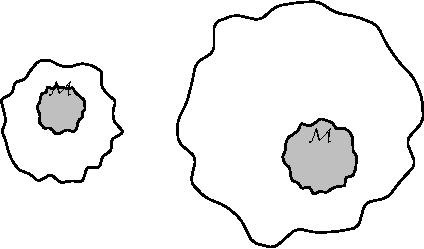
\includegraphics[width=\textwidth]{U:/GitHub/Covariatesets/Diagrams/Identification.pdf}
  \caption{A model $\mathcal{M}$ is a set of structures that forms a proper subset of the class of all structures $\mathcal{S}$. Each structure in $\mathcal{M}$ generates a probability distribution in the class of all probability distributions (of observable variables) $\mathcal{P}$. Then the image $\mathcal{I}$ is the set of all probability distributions that are generated by structures in $\mathcal{M}$.}
  \label{fig:model}
  \end{subfigure}
\begin{subfigure}{0.8\textwidth}
  \centering
  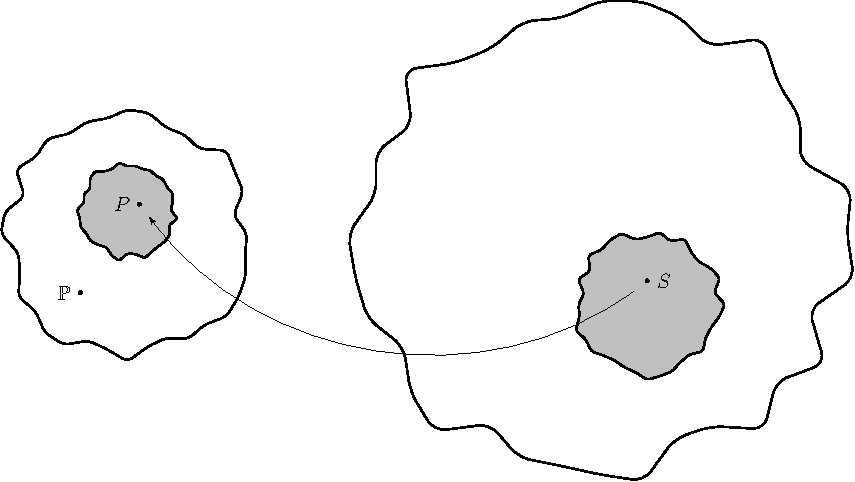
\includegraphics[width=\textwidth]{U:/GitHub/Covariatesets/Diagrams/Observationalrestrictiveness.pdf}
  \caption{A structure $S$ is incompatible with data if it generates a probability distribution (of observable variables) $P$ that is distinct from a realised probability distribution $\mathbb{P}$. If all structures in $\mathcal{M}$ are incompatible with data then $\mathcal{M}$ is said to be observationally restrictive, and is falsified. This condition is equivalent to $\mathbb{P}\in\mathcal{P}\setminus\mathcal{I}$.}
  \label{fig:obs.restrict}
  \end{subfigure}
\caption{Structures, models, probability distributions (of observable variables), and falsifiability.}
\label{fig:models}
\end{figure}
%==================================================%
\begin{figure}[p]
\centering
\begin{subfigure}{0.8\textwidth}
  \centering
  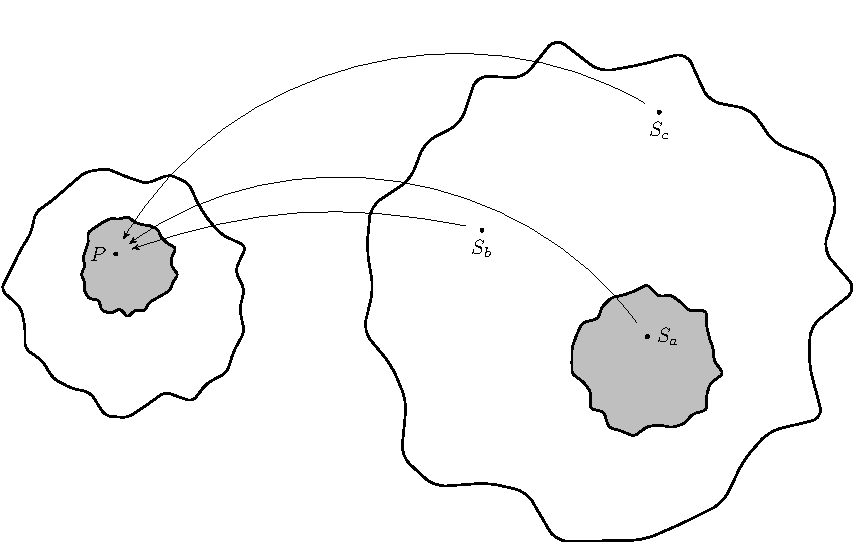
\includegraphics[width=\textwidth]{U:/GitHub/Covariatesets/Diagrams/Pointidentification.pdf}
  \caption{A model $\mathcal{M}$ is said to identify a structure $S$ if the probability distribution (of observable variables) $P$ that is generated by $S$ is distinct from those generated by other structures in $\mathcal{M}$. The structures $S_a$, $S_b$ and $S_c$ are said to be observationally equivalent as they all generate $P$ but $S_b$ and $S_c$ are not admitted by $\mathcal{M}$. As $S_a$ is the only structure that is admitted by $\mathcal{M}$ and that generates $P$, $S_a$ is identified by $\mathcal{M}$. For completeness, $\mathcal{M}$ is said to be uniformly identifying if it identifies each structure that it admits.}
  \label{fig:identify}
  \end{subfigure}
  \begin{subfigure}{0.8\textwidth}
  \centering
  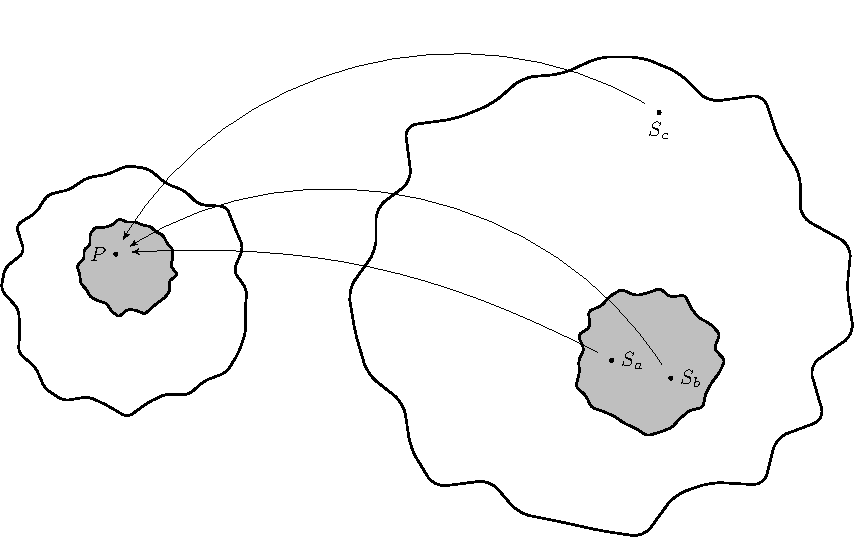
\includegraphics[width=\textwidth]{U:/GitHub/Covariatesets/Diagrams/Setidentification.pdf}
  \caption{As $S_a$ and $S_b$ are observationally equivalent and are both admitted by $\mathcal{M}$ then $\mathcal{M}$ does not identify either $S_a$ or $S_b$. Nonetheless, as $\mathcal{M}$ restricts the set of observationally equivalent structures that generate $P$ to $S_a$ and $S_b$ then $\mathcal{M}$ partially identifies $S_a$ (and $S_b$ to within $\lbrace S_a,S_b\rbrace$).}
  \label{fig:partial}
  \end{subfigure}
\caption{Identification and non-identification of a structure, and partial identification of a structure.}
\label{fig:identification}
\end{figure}
%==================================================%
\begin{figure}[p]
\centering
\begin{subfigure}{0.8\textwidth}
  \centering
  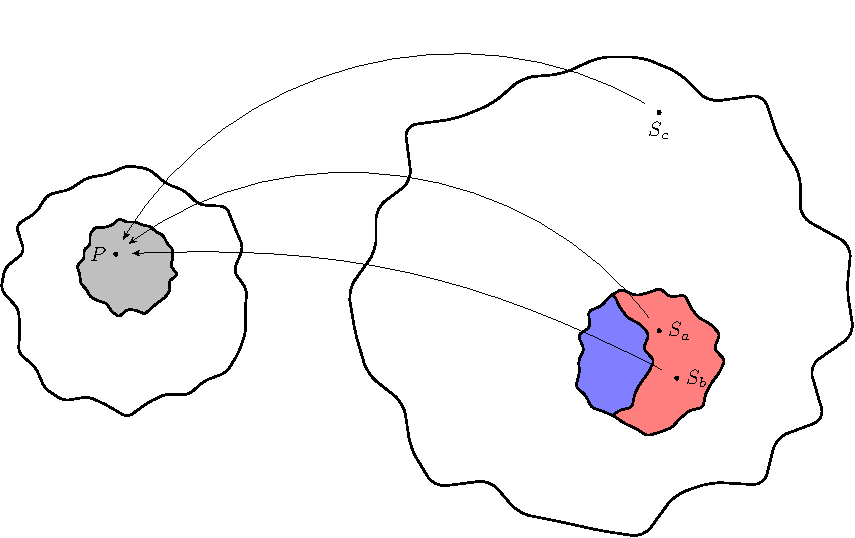
\includegraphics[width=\textwidth]{U:/GitHub/Covariatesets/Diagrams/Characteristic.pdf}
  \caption{A structural characteristic $\Psi$ is a function of a structure $S$. A model $\mathcal{M}$ can be partitioned such that structures in a partition deliver the same value for $\Psi$. Structures in the blue partition $\color{blue}\mathcal{M}$ deliver the value $a$ for $\Psi$, and structures in the red partition $\color{red}\mathcal{M}$ deliver the value $b$ for $\Psi$. If $\Psi$ is constant across all observationally equivalent structures that $\mathcal{M}$ admits then $\mathcal{M}$ is said to identify $\Psi$. As in Figure~\ref{fig:partial} $S_a$ and $S_b$ are not (separately) identified by $\mathcal{M}$ but $\Psi$ is identified by $\mathcal{M}$ since $\Psi(S_a)$ is equal to $\Psi(S_b)$ (is equal to $a$).}
  \label{fig:characteristic}
  \end{subfigure}
  \begin{subfigure}{0.8\textwidth}
  \centering
  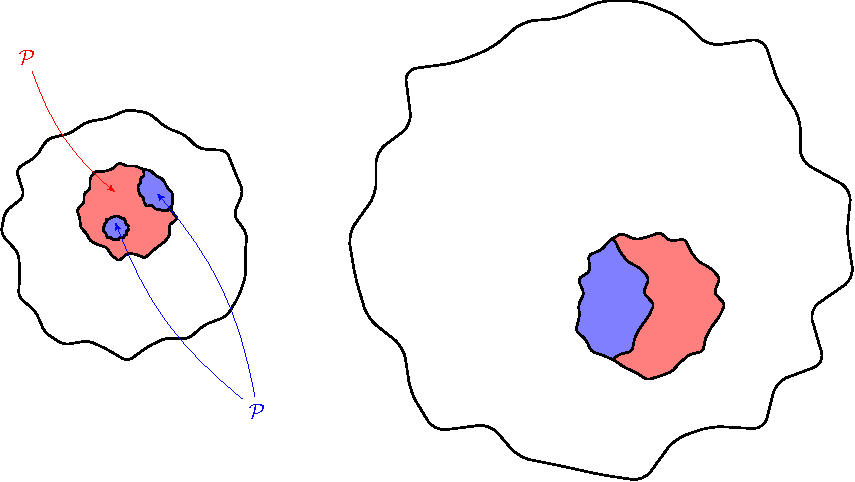
\includegraphics[width=\textwidth]{U:/GitHub/Covariatesets/Diagrams/Uniform.pdf}
  \caption{If $\mathcal{M}$ identifies $\Psi$ for all structures in $\mathcal{M}$ then $\mathcal{M}$ is said to uniformly identify $\Psi$. Whether $\mathcal{M}$ uniformly identifies $\Psi$ can be determined by the existence of an identifying correspondence $G$, a functional. The properties of $G$ are given in the context of Figure~\ref{fig:uniform}. The class of all probability distributions (of observable variables) is partitioned into the blue partition $\color{blue}\mathcal{P}$ and into the red partition $\color{red}\mathcal{P}$. Probability distributions in $\color{blue}\mathcal{P}$ are generated by (potentially many) structures in $\color{blue}\mathcal{M}$, and probability distributions in $\color{red}\mathcal{P}$ are generated by (potentially many) structures in $\color{red}\mathcal{M}$. It is important that $\mathcal{P}$ can be partitioned in this way. $\color{blue}P$ is a probability distribution in $\color{blue}\mathcal{P}$, and $\color{red}P$ is a probability distribution in $\color{red}\mathcal{P}$. Then $\mathcal{M}$ uniformly identifies $\Psi$ if the value of $G(\color{blue}P\color{black})$ is $a$ and if the value of $G(\color{red}P\color{black})$ is $b$, holding for any such $\color{blue}P$ and $\color{red}P$. }
  \label{fig:uniform}
  \end{subfigure}
  \caption{The identification of structural characteristics, and identifying correspondences.}
  \label{fig:characteristics}
\end{figure}
%==================================================%
\begin{figure}[p]
\centering
\begin{subfigure}{0.8\textwidth}
\centering
\caption{A structural characteristic $\Psi$ is a function of a structure $S$. A model $\mathcal{M}$ can be partitioned such that structures in a partition deliver the same value for $\Psi$. Structures in the blue partition $\color{blue}\mathcal{M}$ deliver the value $a$ for $\Psi$, structures in the red partition $\color{red}\mathcal{M}$ deliver the value $b$ for $\Psi$, and structures in the yellow partition $\color{yellow}\mathcal{M}$ deliver the value $c$ for $\Psi$. The class of all probability distributions (of observable variables) $\mathcal{P}$ is partitioned into the blue partition $\color{blue}\mathcal{P}$, into the red partition $\color{red}\mathcal{P}$, into the yellow partition $\color{yellow}\mathcal{P}$ and into the grey partition $\color{gray}\mathcal{P}$. Probability distributions in a colour of $\mathcal{P}$ are generated by (potentially many) structures in the same colour of $\mathcal{M}$; the exception is probability distributions in $\color{gray}\mathcal{P}$ which are generated by (potentially many) structures in $\color{red}\mathcal{M}$ and in $\color{yellow}\mathcal{M}$. $\color{blue}P$ is a probability distribution in $\color{blue}\mathcal{P}$, $\color{red}P$ is a probability distribution in $\color{red}\mathcal{P}$, $\color{yellow}P$ is a probability distribution in $\color{yellow}\mathcal{P}$, and $\color{gray}P$ is a probability distribution in $\color{gray}\mathcal{P}$. $P$ is a probability distribution in $\mathcal{P}$.}
\end{subfigure}
\begin{subfigure}{0.8\textwidth}
  \centering
  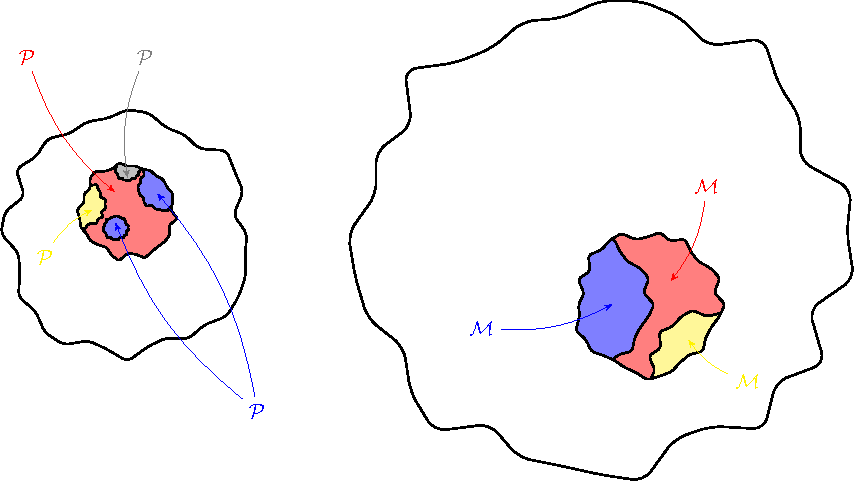
\includegraphics[width=\textwidth]{U:/GitHub/Covariatesets/Diagrams/Partial.pdf}
  \caption{There does not exist an identifying correspondence $G$ that satisfies the required properties of such a functional since $G(\color{gray}P\color{black})$ would need to be multivalued. This is a direct consequence of the colour of $\mathcal{P}$ being strictly greater than the colour of $\mathcal{M}$ ($\mathcal{P}$ can be divided into more partitions than $\mathcal{M}$). As such $\mathcal{M}$ does not identify $\Psi$. Notice that $\mathcal{M}$ does restrict the set of admissible values that $\Psi$ can take for any partition of $\mathcal{P}$ to at most two values ($b$ and $c$ for structures that generate $\color{gray}\mathcal{P}$; all other probability distribuitions in a colour of $\mathcal{P}$ are generated by structures from the same colour of $\mathcal{M}$). Then $\mathcal{M}$ partially identifies $\Psi$ if there exist bounds $G_l$ and $G_u$, functionals of $P$, such that $\Psi$ belongs to the interval $[G_l(P),G_u(P)]$ for any $P$ in $\mathcal{P}$ almost surely. In the context of Figure~\ref{fig:partials} this implies that $a$ is in $[G_l(\color{blue}P\color{black}),G_u(\color{blue}P\color{black})]$ almost surely, that $b$ is in $[G_l(\color{red}P\color{black}),G_u(\color{red}P\color{black})]$ almost surely, that $c$ is in $[G_l(\color{yellow}P\color{black}),G_u(\color{yellow}P\color{black})]$, and that $\lbrace b,c\rbrace$ is in $[G_l(\color{gray}P\color{black}),G_u(\color{gray}P\color{black})]$ almost surely. When $[G_l(P),G_u(P)]$ cannot be made any tighter without $\Psi$ lying outside of these bounds for at least one $P$ in the image $\mathcal{I}$ that is the set of all probability distributions that are generated by structures in $\mathcal{M}$ then these bounds are said to be sharp.}
  \label{fig:partial1}
  \end{subfigure}
  \caption{Partial identification of structural characteristics.}
  \label{fig:partials}
\end{figure}
%==================================================%
%% Bibliography.
\bibliographystyle{chicago}
\bibliography{\details Bibliography}
\end{document}
